\documentclass[11pt, oneside]{report}   	% use "amsart" instead of "article" for AMSLaTeX format
\usepackage{geometry}                		% See geometry.pdf to learn the layout options. There are lots.
\geometry{letterpaper}                   		% ... or a4paper or a5paper or ... 
%\geometry{landscape}                		% Activate for for rotated page geometry
%\usepackage[parfill]{parskip}    		% Activate to begin paragraphs with an empty line rather than an indent
\usepackage{graphicx}				% Use pdf, png, jpg, or eps� with pdflatex; use eps in DVI mode
\usepackage{float}							       % TeX will automatically convert eps --> pdf in pdflatex		
\usepackage{epstopdf}
\usepackage{amssymb}
\usepackage{amsmath}
\usepackage{titling}
\usepackage{appendix}

\usepackage[framed,numbered,autolinebreaks,useliterate]{mcode}
\newfloat{code}{H}{myc}
\setcounter{MaxMatrixCols}{20}


\newcommand{\subtitle}[1]{%
  \posttitle{%
    \par\end{center}
    \begin{center}\large#1\end{center}
    \vskip0.5em}%
}

\newcommand{\footnotewithref}[2]{
\footnote{#2}
\newcounter{#1}
\setcounter{#1}{\value{footnote}}
}
\newcommand{\footnoteref}[1]{
\footnotemark[\value{#1}]
}

\title{Celestial to Terrestrial Transformation}
\subtitle{A CIO Based Matrix Algebra Approach using MATLAB}
\author{Abel Brown, PhD}
\date{}							% Activate to display a given date or no date
\begin{document}
\maketitle
\tableofcontents


\chapter{Definitions}
Please note that the contents of this first chapter are pulled \emph{directly} from the IERS technical notes 32/36 chapter 5, David Vallado's paper (AAS 06-134), and excerpts from the SOFA library pages (iausofa.org). These references can be found in the associated "refs" folder.  
\section{Overview}
The transformation to be used to relate the International Terrestrial Reference System (ITRS) to the Geocentric Celestial Reference System (GCRS) at the date $t$ of the observation can be written as:
\begin{equation}
\label{eqn:gcrs2itrs}
[GCRS] = Q(t)R(t)W(t) [ITRS]
\end{equation}
where $Q(t)$, $R(t)$, and $W(t)$ are the transformation matrices arising from the motion of the celestial pole in the celestial reference system, from the rotation of the Earth around the axis associated with the pole, and from polar motion respectively.  Note that Eq. (\ref{eqn:gcrs2itrs}) is valid for any choice of celestial pole and origin on the equator of that pole.  The definition of the GCRS and ITRS and the procedures for the ITRS to GCRS transformation that are provided in this document comply with the IAU 2000/2006 resolutions.  Numerical values contained in this document are compliant with the IAU 2006 precession.  More detailed explanations about the relevant concepts, software, and IERS products corresponding to the IAU 2000 resolutions can be found in IERS Technical Notes 29, 32, and 36  

\begin{figure}
\centering
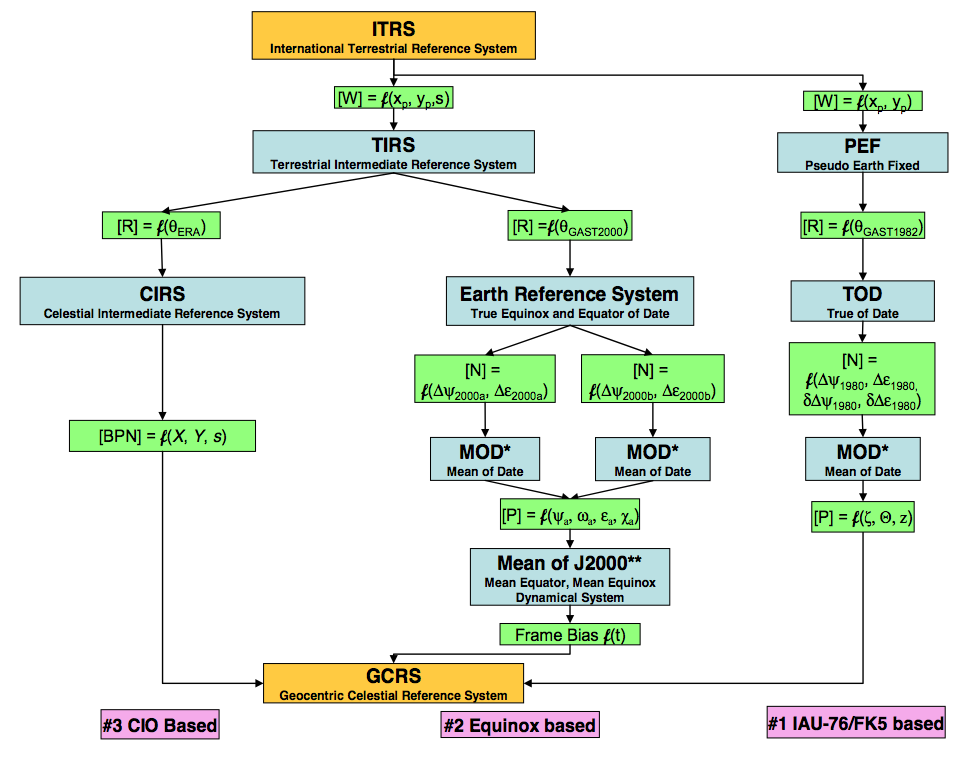
\includegraphics[scale=0.40]{C2T_coord_xforms.png}
\caption{\emph{Celestial to Terrestrial Coordinate Transformations}.  Three general approaches (and two variations) transform vectors between terrestrial (ITRS) and celestial coordinate systems (GCRS).  Although names (e.g polar motion, mean-of-date, etc) are the same, the formulae are different.  IAU-76/FK5 precession/nutation corrections are found in the EOP data.  There are also two approaches for the equinox-based precession/nutation models, IAU-2000A and IAU 2000B.  Image ref: Vallado AAS 06-134.}
\label{fig:c2t_methods}
\end{figure}

The \emph{Celestial Intermediate Origin} (CIO) based method is the newest technique, but is also most different from the previous equinox and IAU76/FK5 implementations. This CIO based method effectively eliminates the distinctions of the `equinox' and `mean position of date'. The process rests with the determination of the CIO coordinates; $X$, $Y$, and $s$. These are the \emph{Celestial Intermediate Pole} (CIP) coordinates in the GCRS.  Sidereal time is replaced by \emph{Earth Rotation Angle} (ERA).  The Greenwich meridian is replaced by an International Terrestrial Reference Frame (ITRF), and a Terrestrial Intermediate Origin (TIO) is used for the rotation frame.  These, in turn, form a transformation matrix that is used to convert vectors between systems.  There are no ``mean'' positions - only the \emph{International Celestial Reference Frame} (ICRF) and true positions - in this system.  See figure (\ref{fig:c2t_methods}) for more details.


%\subsection{Definitions of $Q(t)$, $R(t)$, and $W(t)$}

\section{Transformation matrix for polar motion}
The transformation matrix arising from polar motion (i.e. relating TIRS and ITRS) can be expressed as:
\begin{equation}
\label{eqn:polar_motion_matrix}
W_{TIRS \rightarrow ITRS} (t) = R_1(-y_p) \cdot R_2(-x_p) \cdot R_3(s')
\end{equation}
where $x_p$ and $y_p$ are the �polar coordinates� of the CIP in the ITRS and $s'$ being a quantity, named ``TIO locator'', which provides the position of the \emph{Terrestrial Intermediate Origin} (TIO) on the equator of the CIP corresponding to the kinematical definition of the ``non-rotating'' origin (NRO) in the ITRS when the CIP is moving with respect to the ITRS due to polar motion.  The use of the quantity $s'$, which was neglected in the classical form prior to 1 January 2003, is necessary to provide an exact realization of the ``instantaneous prime meridian'' (designated by ``TIO meridian'').

The quantity $s'$ (i.e. the TIO locator) appearing in Eq. (\ref{eqn:polar_motion_matrix}) is sensitive only to the largest variations in polar motion. Some components of $s'$ have to be evaluated, in principle, from the measurements and can be extrapolated using the IERS data. Its main component can be written as 
$s' = -0.0015 (a^2_c/1.2+a^2_a) t$
 where $a_c$ and $a_a$ are the average amplitudes (in arc-seconds) of the Chandlerian and annual wobbles, respectively, in the period considered (Capitaine et al., 1986). The value of $s'$ will therefore be less than 0.4 mas through the next century, even if the amplitudes for the Chandlerian and annual wobbles reach values of the order of $0.5''$ and $0.1''$, respectively. Using the current mean amplitudes for the Chandlerian and annual wobbles (Lambert and Bizouard, 2002) gives $s'$ in micro arc-seconds ($\mu$as) as:
\begin{equation}
\label{eqn:s_prime}
s' = -47 \cdot t_c
\end{equation}
where $t_c$ is in Julian centuries since J2000 referenced to Terrestrial Time (TT)\footnotewithref{def:tc}{That is, $t_c = ( 2400000.5 - 2451545 + $ fMJD$_{TT})/36525 $.}
%$\footnote{Test values: fMJD$_{TT}$ = 54195.5007544,  $t_c = 0.0725804$}.  

\section{CIO based transformation matrix for Earth rotation}
The CIO based transformation matrix arising from the rotation of the Earth around the axis of the CIP (i.e. relating CIRS and TIRS), can be expressed as:
\begin{equation}
\label{eqn:era}
R_{CIRS \rightarrow TIRS}(t) = R_3(ERA)
\end{equation}
where ERA is the Earth Rotation Angle between the CIO and the TIO at date t on the equator of the CIP, which provides a rigorous definition of the sidereal rotation of the Earth.

The conventional relationship defining UT1 in radians from the Earth Rotation Angle (ERA) to be used is that given by Capitaine et al. (2000):
\begin{equation}
\label{def:era}
ERA(T_{UT1}) = 2\pi(F_{UT1} + 0.7790572732640 + 0.00273781191135448 \cdot T_{UT1})
\end{equation}
where $F_{UT1}$ is the UT1 Julian day fraction and $T_{UT1} =$Julian UT1 date - $2451545.5$.  Note that $ERA$ should be normalized between 0 and $2\pi$.   This definition of UT1 based on the CIO is insensitive at the micro-arcsecond level to the precession-nutation model and to the observed celestial pole offsets.  Note also that, for 0h UT1, the UT1 Julian day fraction in Eq. (\ref{def:era}) is 0.5.  Similarly to polar motion, additional components should be added to the values published by the IERS for UT1 and LOD to account for the effects of ocean tides and libration\footnote{See UTLIBR.F provided by the IERS at http://tai.bipm.org/iers/}.

\section{Transformation matrix for the CIP celestial motion}
The CIO based transformation matrix arising from the motion of the CIP in the GCRS (i.e. relating GCRS and CIRS), can be expressed as:
\begin{equation}
\label{def:c}
Q_{GCRS \rightarrow CIRS}(t) = R_3(-(E+s)) \cdot R_2(d) \cdot R_3(E);
\end{equation}
E and d being such that the coordinates of the CIP in the GCRS are:
\begin{equation}
\label{def:xyz}
X = \sin(d) \cos(E), \;\;\;\;\;\;Y = \sin(d)\sin(E),\;\;\;\;\;\; Z = \cos(d)
\end{equation}
and s being a quantity, named ``CIO locator'', which provides the position of the CIO on the equator of the CIP corresponding to the kinematical definition of the NRO in the GCRS when the CIP is moving with respect to the GCRS, between the reference epoch and the date $t$ due to precession and nutation.  Thus, provided $X$ and $Y$ in radians, the quantities E and d are:
\begin{equation}
\label{def:ed}
E = atan2(Y,X), \;\;\;\;\;\; d = atan\left(\sqrt{\frac{X^2 + Y^2}{1 - (X^2 + Y^2)}}\right)
\end{equation} 

\section{Expression for $X$, $Y$, and $s$}

The coordinates of the CIP in the GCRS to be used for the parameters $X$ and $Y$ appearing in Eq. (\ref{def:ed}) can be given by developments as function of time of those quantities. Developments valid at the microarcsecond level, based on the IAU 2006 precession and IAU 2000A nutation and on their corresponding pole and equinox offsets at J2000.0 with respect to the pole of the GCRS have been computed (Capitaine and Wallace, 2006). They replace the previous developments based on the IAU 2000 model for precession-nutation and frame biases that had been provided by Capitaine et al. (2003a) and in the IERS 2003 Conventions.

The IAU 2006/2000A developments for $X$, $Y$, and $s$ in microarcseconds, are as follows:

\begin{equation}
\label{def:X}
\begin{split}
X = & -16617 t^0 + 2004191898 t^1 - 429782.9 t^2 - 198618.34 t^3 + 7.578 t^4 + 5.9285 t^5 \\
 &+ \sum_i^{1306} \: [\: s_{x,0,i} \: \sin(ARG) + c_{x,0,i} \: \cos(ARG)\: ] \cdot t^0 \\
& + \sum_j^{253} \: [\: s_{x,1,j} \: \sin(ARG) + c_{x,1,j} \: \cos(ARG)\: ] \cdot t^1 \\
& + \sum_k^{36} \: [\: s_{x,2,k} \: \sin(ARG) + c_{x,2,k} \: \cos(ARG)\: ] \cdot t^2 \\
& + \sum_l^4\: [\: s_{x,3,l} \: \sin(ARG) + c_{x,3,l} \: \cos(ARG)\: ] \cdot t^3 \\
& + \sum_m^1 \: [\: s_{x,4,m} \: \sin(ARG) + c_{x,4,m} \: \cos(ARG)\: ] \cdot t^4 \\
\end{split}
\end{equation}


\begin{equation}
\label{def:Y}
\begin{split}
Y = & - 6951t^0 - 25896 t^1 - 22407274.7 t^2 + 1900.59 t^3 + 1112.526 t^4 + 0.1358 t^5 \\
 &+ \sum_i^{962} \: [\: s_{y,0,i} \: \sin(ARG) + c_{y,0,i} \: \cos(ARG)\: ] \cdot t^0 \\
& + \sum_j^{277} \: [\: s_{y,1,j} \: \sin(ARG) + c_{y,1,j} \: \cos(ARG)\: ] \cdot t^1 \\
& + \sum_k^{30} \: [\: s_{y,2,k} \: \sin(ARG) + c_{y,2,k} \: \cos(ARG)\: ] \cdot t^2 \\
& + \sum_l^5\: [\: s_{y,3,l} \: \sin(ARG) + c_{y,3,l} \: \cos(ARG)\: ] \cdot t^3 \\
& + \sum_m^1 \: [\: s_{y,4,m} \: \sin(ARG) + c_{y,4,m} \: \cos(ARG)\: ] \cdot t^4 \\
\end{split}
\end{equation}

\begin{equation}
\label{def:s}
\begin{split}
s = & + 94.0t^0 + 3808.65 t^1 - 122.68 t^2 - 72574.11 t^3 + 27.98 t^4 + 15.62 t^5\\
 &+ \sum_i^{33} \: [\: s_{s,0,i} \: \sin(ARG) + c_{s,0,i} \: \cos(ARG)\: ] \cdot t^0 \\
& + \sum_j^{3} \: [\: s_{s,1,j} \: \sin(ARG) + c_{s,1,j} \: \cos(ARG)\: ] \cdot t^1 \\
& + \sum_k^{25}  \: [\: s_{s,2,k} \: \sin(ARG) + c_{s,2,k} \: \cos(ARG)\: ] \cdot t^2 \\
& + \sum_l^4       \: [\: s_{s,3,l} \: \sin(ARG) + c_{s,3,l} \: \cos(ARG)\: ] \cdot t^3 \\
& + \sum_m^1     \: [\: s_{s,4,m} \: \sin(ARG) + c_{s,4,m} \: \cos(ARG)\: ] \cdot t^4 \\
&  - \frac{XY}{2}\\ 
\end{split}
\end{equation}
the parameter t being Julian centuries since J2000 referenced to Terrestrial Time (TT) given by expression $\langle$\footnoteref{def:tc}$\rangle$ and ARG (a function of t) constructed from the fundamental arguments of the nutation theory, whose expressions are given by Tab. \ref{tab:fund_args}. 

The full IAU 2000/2006 series for $X$, $Y$, and $s$ are available electronically on the IERS Conventions Center website
\footnotewithref{xyscoeffs}{ftp://tai.bipm.org/iers/convupdt/chapter5, tab5.2a.txt, tab5.2b.txt, and tab5.2d.txt }. 
An extract for the largest non-polynomial terms in $X$ and $Y$ is given in tables \ref{tab:X_coeffs} and \ref{tab:Y_coeffs}.

%The numerical values of the coefficients of the polynomial part of X and Y are derived from the development as a function of time of the precession in longitude and obliquity and pole offset at J2000.0 and the amplitudes (Fourier and Poisson coefficients) are derived from the amplitudes of the precession and nutation series. The amplitudes (as,0)i, (bc,0)i of the sine and cosine terms in X and Y respectively are equal to the amplitudes Ai ? sin ?0 and Bi of the series for nutation in longitude and obliquity, except for a few terms in each coordinate X and Y which contain a contribution from crossed- nutation effects. The coordinates X and Y contain Poisson terms in $t sin$, $t cos$, $t^2 sin$, $t^2 cos$, ... which originate from crossed terms between precession and nutation.

\begin{table}
\label{tab:X_coeffs}
\begin{tabular}{cccccccccccccccccc}
 X\\ 
\hline
&&  $s_{x,0,i}$  &   $c_{x,0,i}$ \\
&1   & -6844318.44       & 1328.67   & 0    &0 &   0    &0 &   1   & 0 &   0   & 0  &  0   & 0  &  0   & 0 &   0   & 0 \\
 &   2  &   -523908.04    &    -544.75   & 0   & 0  &  2  & -2 &   2  &  0  &  0  &  0  &  0  &  0  &  0  &  0   & 0  &  0 \\
 &   3    &  -90552.22    &     111.23    &0  &  0    &2 &   0   & 2 &   0   & 0  &  0   & 0  &  0  &  0 &   0   & 0 &   0 \\
&$\ldots$ &&&&&&&&&&&&&&&& \\
& &        $s_{x,1,j}$  &   $c_{x,1,j}$  &  \\ 
&1307   &    -3309.73    &  205833.11  &  0  &  0  &  0  &  0 &   1   & 0 &   0  &  0 &   0  & 0  &  0  &  0 &   0  &  0 \\
 &1308    &     198.97   &    12814.01   & 0 &   0    & 2 &  -2   & 2 &   0   & 0 &   0   & 0 &   0  &  0 &   0  &  0 &   0 \\
&$\ldots$ &&&&&&&&&&&&&&&& \\
& &        $s_{x,2,k}$  &   $c_{x,2,k}$  & \\
&1560  &      2037.98   &       81.46  &  0 &   0 &   0 &   0  &  1 &   0 &  0  &  0  &  0 &   0 &   0  &  0  &  0 &   0  \\
&$\ldots$ &&&&&&&&&&&&&&&& \\
\end{tabular}
\caption{Series coefficients of $X$ with associated fundamental argument multipliers.}
\end{table}

\begin{table}
\label{tab:Y_coeffs}
\begin{tabular}{cccccccccccccccccc}
Y & &        &  &  &&&&&&&&&&&&&\\ 
\hline
&&$s_{y,0,i}$  &   $c_{y,0,i}$ \\
&1 &        1538.18  &   9205236.26 &   0  &  0 &   0 &   0  &  1  &  0  &  0 &   0 &   0 &   0 &   0 &   0 &   0  & 0\\ 
&2  &      -458.66    &  573033.42    &0    & 0   & 2   & -2  &   2   &  0 &   0 &   0 &   0 &   0 &   0 &   0 &   0 &   0\\
&3  &       137.41    &   97846.69     & 0   & 0   & 2    &0    & 2    & 0   & 0   & 0   & 0   & 0   & 0   & 0   & 0   & 0 \\
&$\ldots$ &&&&&&&&&&&&&&&& \\
 &&        $s_{y,1,j}$  &   $c_{y,1,j}$  &  \\ 
&963  &    153041.79    &     853.32  &  0  &  0 &   0 &   0  &  1 &   0 &   0  &  0  &  0 &   0 &   0 &   0 &   0 &   0\\
&964    &   11714.49    &    -290.91 &   0  &  0 &   2  & -2  &  2  &  0 &   0 &   0  &  0  &  0 &   0  &  0  &  0  &  0 \\
&$\ldots$ &&&&&&&&&&&&&&&& \\
 &&        $s_{y,2,k}$  &   $c_{y,2,k}$  &  \\
&1240     &    120.56  &     -2301.27  &  0 &   0  &  0  &  0  &  1 &   0 &   0 &   0 &   0  &  0 &   0  &  0 &   0 &   0 \\
&$\ldots$ &&&&&&&&&&&&&&&& \\
\end{tabular}
\caption{Series coefficients of Y with associated fundamental argument multipliers}
\end{table}


\begin{table}
\label{tab:s_coeffs}
\begin{tabular}{cccccccccccccccccc}
s & &        &  &  &&&&&&&&&&&&&\\ 
\hline
&&$s_{s,0,i}$  &   $c_{s,0,i}$ \\
 &   1  &      -2640.73    &       0.39 &   0  &  0 &   0 &   0  &  1  &  0 &   0  &  0  &  0 &   0 &   0 &   0 &   0 &   0 \\
 &   2    &     -63.53      &     0.02  &  0   & 0  &  0   & 0   & 2  &  0  &  0   & 0  &  0  &  0  &  0  &  0  &  0   & 0  \\
 &   3      &   -11.75    &      -0.01  &  0 &   0  &  2 &  -2   & 3 &   0   & 0  &  0  &  0 &   0  &  0  &  0  &  0 &   0 \\
 &$\ldots$ &&&&&&&&&&&&&&&& \\
 &&        $s_{s,1,j}$  &   $c_{s,1,j}$  &  \\ 
&34   &       -0.07   &        3.57   & 0  &  0 &   0  &  0  &  2  &  0  &  0  &  0 &   0   & 0  &  0   & 0  &  0  &  0 \\
 &  35    &       1.73 &         -0.03  &  0 &   0  &  0  &  0 &   1 &   0 &   0 &   0 &   0  &  0  &  0 &   0  &  0 &   0 \\
   
&$\ldots$ &&&&&&&&&&&&&&&& \\
 &&        $s_{s,2,k}$  &   $c_{s,2,k}$  &  \\
&37   &      743.52    &      -0.17   & 0  &  0    &0  &  0  &  1 &   0  &  0  &  0  &  0  &  0 &   0  &  0  &  0 & 0 \\
&$\ldots$ &&&&&&&&&&&&&&&& \\
\end{tabular}
\caption{Series coefficients of S with associated fundamental argument multipliers}
\end{table}

\section{The fundamental arguments of nutation theory}
In order to compute $ARG(t)$ of equations \ref{def:X}, \ref{def:Y}, and \ref{def:s} the fundamental arguments of nutation theory must be evaluated.  Each  of the 14 fundamental arguments of nutation theory (Delaunay variables) can be posed as a 4$^{th}$ order polynomial in $t$, the coefficients of which are provided in Table \ref{tab:fund_args}.  Terms $F_1 \ldots F_5$ are called lunisolar and terms $F_6 \ldots F_14$ are planetary.   Each set of Fourier and Poisson coefficients, \{$s_i$,$c_i$\}$_{X,Y,s}$, are associated with a set of 14 multipliers (or expressions), $a_i = \{1, 0, 0, -2, \ldots \}$, one for each fundamental argument.  And so, the $ARG(t)$ term associated with \{$s_i$,$c_i$\}$_{X,Y,s}$ is computed as 
\begin{equation}
\label{eqn:arg}
ARG_i(t) = \sum_k^{14} a_{i,k} \cdot F_k(t)
\end{equation}
\begin{table}
\begin{tabular}{l*{5}{c}}
\label{tab:fund_args}
&$t^0$&$t^1$&$t^2$&$t^3$&$t^4$ \\
\hline
$F_1$ & 485868.249036      &1717915923.2178 & 31.8792  & 0.051635  & -0.00024470\\
$F_2$ & 1287104.793048   & 129596581.0481  & -0.5532    & 0.000136   & 0.00001149 \\
$F_3$ & 335779.526232     & 1739527262.8478     &  -12.7512   & -0.001037   & 0.00000417 \\
$F_4$ & 1072260.703692    & 1602961601.2090   & -6.3706   &  0.006593    &  -0.00003169 \\
$F_5$ & 450160.398036   &   -6962890.5431    &   7.4722    &   0.007702     &   -0.00005939 \\
$F_6$ & 4.402608842  &  2608.7903141574  &     0.0     &      0.0      &  0.0 \\
$F_7$ & 3.176146697   & 1021.3285546211  &  0.0    &  0.0        & 0.0 \\
$F_8$ & 1.753470314   & 628.3075849991  &    0.0     &    0.0     &      0.0 \\
$F_9$     & 6.203480913   &   334.0612426700  &    0.0    &  0.0     &  0.0 \\
$F_{10}$ & 0.599546497  &     52.9690962641 &    0.0   &    0.0     &      0.0 \\
$F_{11}$ & 0.874016757   &  21.3299104960  & 0.0   & 0.0    &  0.0 \\
$F_{12}$ &5.481293872   & 7.4781598567 &  0.0   &   0.0     &    0.0 \\
$F_{13}$ & 5.311886287   &  3.8133035638  & 0.0     &    0.0     &     0.0 \\
$F_{14}$ & 0.0  & 0.024381750   &  0.00000538691 &   0.0      &  0.0 \\

\end{tabular}
\caption{Polynomial coefficients for each of the lunisolar and planetary fundamental arguments.}
\end{table}

\chapter{Implementation}
Much of the work involved in the Celestial to Terrestrial transformation lyes in the series computation of $X$, $Y$, and $s$.  While large summation might not pose issues in FORTRAN or C, such traditional implementation are not well suited for MATLAB.  The main focus of this chapter is to reformulate the calculations of the CIP coordinates using matrix algebra.  This matrix formulation reduces the notational complexities and can provide scalability improvements for coordinate transformations performed in MATLAB.   

\section{Matrix Algebra Formulation}

The number of terms in each of the $X$,$Y$, and $s$ series are defined as:
\begin{equation}
\label{def:Nxys}
\begin{split}
N_X = & [1306, 253, 36, 4, 1] \\
N_Y = & [962, 277, 30, 5, 1] \\
N_s = & [33, 3, 25, 4, 1] \\
\end{split}
\end{equation}
where $sum(N_X) = 1600$, $sum(N_Y) = 1275$, and $sum(N_s) = 66$.  Here for example $N_X(1)$ defines the number of $t^0$ $X$ series terms (non polynomial terms), $N_X(2)$ the number of $t^1$ $X$ series terms,  and so on (see Eq. \ref{def:X}, \ref{def:Y}, and \ref{def:s}).

The series coefficient vectors $\vec{C}_{X,Y,s}$ and $\vec{S}_{X,Y,s}$ are defined as:

\begin{align}
\begin{matrix}
 \vec{C_X} &= \left[\!
\begin{array}{c}
      c_{x,1} \\
      c_{x,2}\\
      \vdots \\
      c_{x,1600}\\
    \end{array}
    \!\right]                                     & 
      \vec{S_X} &= \left[\!
\begin{array}{c}
      s_{x,1} \\
      s_{x,2}\\
      \vdots \\
      s_{x,1600}\\
    \end{array}
    \!\right]                                     \\
    &                                              \\
 \vec{C_Y} &= \left[\!
\begin{array}{c}
      c_{y,1} \\
      c_{y,2}\\
      \vdots \\
      c_{y,1275}\\
    \end{array}
    \!\right]                                     & 
      \vec{S_Y} &= \left[\!
\begin{array}{c}
      s_{y,1} \\
      s_{y,2}\\
      \vdots \\
      s_{y,1275}\\
    \end{array}
    \!\right]                                     \\
    &                                               \\
 \vec{C_s} &= \left[\!
\begin{array}{c}
      c_{s,1} \\
      c_{s,2}\\
      \vdots \\
      c_{s,66}\\
    \end{array}
    \!\right]                                     & 
      \vec{S_s} &= \left[\!
\begin{array}{c}
      s_{s,1} \\
      s_{s,2}\\
      \vdots \\
      s_{s,66}\\
    \end{array}
    \!\right]    
\end{matrix}
\end{align}
and notice no distinction is made between coefficients of varying powers $t$ as such information is maintained by $N_{X,Y,s}$.

Suppose we wish to evaluate the $X$,$Y$, and $s$ series at $N$ times
\begin{equation}
\vec{t} = \begin{pmatrix} t_1, t_2, \ldots, t_N\end{pmatrix}
\end{equation}
then the 14 fundamental arguments must be computed at each time $t_i$.  Let $F\left(\vec{t}\:\right)$ be the matrix of having evaluated $F_k(t_i)$ for $k = \{1 \ldots 14\}$ and $i = \{1 \ldots N\}$.  Thus we have 
\begin{equation}
F\left(\vec{t}\:\right) = 
\begin{pmatrix}
F_{1,1} & F_{1,2} & \cdots & F_{1,14} \\
  F_{2,1} & F_{2,2} & \cdots & F_{2,14} \\
  \vdots  & \vdots  & \ddots & \vdots  \\
  F_{N,1} & F_{N,2} & \cdots & F_{N,14}
\end{pmatrix} _{N \times 14}
\end{equation}
where the $i^{th}$ row of $F$ contains the 14 fundamental arguments evaluated at time $t_i$.  

Upon inspection, the definition of $ARG(t)$ (Eq. \ref{eqn:arg}) is simply a dot product of the expression vector and the fundamental arguments at some time $t$. Consider momentarily the $X$ series and note that for each time $t_i$ there are 1600 $ARG$ terms.  That is, at each time $t_i$, each series coefficient pair $\{c_j, s_j\}_{X,Y,s}$ is associated with it's own $ARG_{j}$ term.  Therefore expression matrices $A_{X,Y,s}$ are defined containing the multipliers for each coefficient pair:
\begin{equation}
A_X = \begin{pmatrix} 
0&0&0&0&1&0&0&0&0&0&0&0&0&0 \\
0   & 0  &  2  & -2 &   2  &  0  &  0  &  0  &  0  &  0  &  0  &  0   & 0  &  0 \\
0  &  0    &2 &   0   & 2 &   0   & 0  &  0   & 0  &  0  &  0 &   0   & 0 &   0 \\
&\ldots\\
0  &  0 &   0 &   0  &  1 &   0 &   0  &  0  &  0 &   0 &   0 &   0 &   0 &   0 \\
0 &   0    & 2 &  -2   & 2 &   0   & 0 &   0   & 0 &   0  &  0 &   0  &  0 &   0 \\
& \ldots\\
0 &   0 &   0 &   0  &  1 &   0 &  0  &  0  &  0 &   0 &   0  &  0  &  0 &   0  \\
&\ldots \\
\end{pmatrix}_{1600\times 14}
\end{equation}
where the j$^{th}$ row corresponds to coefficients $\{c_j, s_j\}_{X,Y,s}$.  Likewise, the expression matrices $A_Y$, and $A_s$ are defined accordingly.  And, thus the $ARG$ dot products at each time $t_i$ for $X$, $Y$, and $s$ are formed via matrix-matrix multiplication as:
\begin{equation}
\label{def:ARGXYs}
ARG = (A\:F^T)^T
\end{equation} 
So for example, $ARG_{X} $ would be
\begin{equation}
(A_{X}F^T)^T = 
\begin{pmatrix}
\phi_{1,1} & \phi_{1,2} & \cdots & \phi_{1,1600} \\
  \phi_{2,1} & \phi_{2,2} & \cdots & \phi_{2,1600} \\
  \vdots  & \vdots  & \ddots & \vdots  \\
  \phi_{N,1} & \phi_{N,2} & \cdots & \phi_{N,1600}
\end{pmatrix} _{N \times 1600}
\end{equation} 
where the i$^{th}$ row corresponds to time $t_i$.  Similarly $ARG_{Y}$ has dimensions $N \times 1275$ and $ARG_{s}$ has dimensions $N \times 66$.  It's worth computing a few $\phi_{i,j}$ by hand to ensure that the $ARG$ matrices are fully understood.

There is one more matrix required to compute the series summations.  This matrix makes sure that each $\sin$ and $\cos$ term is multiplied by the correct power of $t$.  Therefore, we construct a matrix $T$ having the same dimensions as ARG where the i$^{th}$ row contains the appropriate powers of $t_i$ such that 
\begin{equation}
T_i = 
\begin{pmatrix}
t_i^0 & \ldots & t_i^0 & t_i^1 & \ldots & t_i^1 &t_i^2 & \ldots & t_i^2 & t_i^3 & \ldots & t_i^3 & t_i^4 & \ldots & t_i^4  
\end{pmatrix}
\end{equation}
Clearly, according to the definitions of $N_{X,Y,s}$ (Eq. \ref{def:Nxys}), $T_i$ corresponding with the $X$ series would contain 1306 $t_i^0$ terms, 253 $t_i^1$ terms, and so on.

We are now ready to compute the $X$, $Y$, and $s$ series.  In general, each series is simply computed as
\begin{equation}
\label{eqn:seriessum}
 P + [\cos(ARG) \circ T] \: \vec{C} +  [\sin(ARG) \circ T] \: \vec{S}
\end{equation}
where the $\circ$ indicates element-wise matrix multiplication (\emph{not} matrix-matrix multiply) where $(A \circ B)_{ij} = (A)_{ij}(B)_{ij}$\footnotewithref{matlabdotmult}{This is equivalent in matlab to $A \:.\!*B$ }\!\!$^,$\!\! \footnotewithref{hadarmad}{$A \circ B$ is also known as a \emph{Hadamard} product}.  So the $X$ series for $\vec{t}$ would be computed as 
\begin{equation}
\label{eqn:seriessumx}
\begin{split}
X(\vec{t}\:)  & =  P_{X}(\vec{t}\:) + [\cos(ARG_{X}) \circ T_{X}] \: \vec{C}_{X}  +  [ \sin(ARG_X) \circ T_{X}] \: \vec{S}_{X}\\
\end{split}
\end{equation} 
having dimensions $N \times 1$ where $P_{X,Y,s}(\vec{t}\:)$ are the polynomial expressions defined by equations \ref{def:X}, \ref{def:Y}, and \ref{def:s} evaluated at each time $t_i \in t$.

 
%(A_{X}F(\vec{t}\:)^T) \circ T_{X}] \: \vec{C}_{X} +  [\sin(A_{X}F(\vec{t}\:)^T) \circ T_{X}] \: \vec{S}_{X} \\
%Y(\vec{t}\:)  & =  P_{Y}(\vec{t}\:) + [\cos(ARG_{Y}) \circ T_{Y}] \: \vec{C}_{Y}  +  [ \sin(ARG_Y) \circ T_{Y}] \: \vec{S}_{Y} \\
%s(\vec{t}\:)  & =  P_{s}(\vec{t}\:) + [\cos(ARG_{s}) \circ T_{s}] \: \vec{C}_{s}  +  [ \sin(ARG_s) \circ T_{s}] \: \vec{S}_{s}  \\


\subsection{MATLAB Implementation Details}
Now that a matrix formulation is in place it is rather trivial to implement in MATLAB.  At this point, making sure each function uses the correct time reference system and outputs the correct units will be the most challenging aspect.  

As demonstrated by the generalized series summation (Eq. \ref{eqn:seriessum}) a single generalized algorithm can be constructed that agnostically computes the X,Y,s series given the appropriate matrices as discussed in the previous section.  The following code listing does just that:
\begin{code}
\begin{lstlisting}
	   function seriesSum = seriesImpl(t,F,A,N,c,s)

            % compute powers of t for Poisson terms [Nx{1600,1275,66}]
            T = [                              ...
                    t(:,ones(1,N(1))).^0 ...
                    t(:,ones(1,N(2))).^1 ...
                    t(:,ones(1,N(3))).^2 ...
                    t(:,ones(1,N(4))).^3 ...
                    t(:,ones(1,N(5))).^4 ...
            ];
        
            % compute the argument [Nx{1600,1275,66}]
            ARG = (A*F')';
            
            % the sum of the series at each time [Nx1]
            seriesSum = (sin(ARG).*T)*s + (cos(ARG).*T)*c;
            
        end
\end{lstlisting}
\end{code}

Equipped with engine for computing each of the series terms, $X$,$Y$, and $s$ can be easily computed.  The following listing is an object method belonging to the IERS.m class.  The IERS.m has internally defined the relevant static quantities (mostly matrices and a few constants) necessary for the computation of the transformation
\begin{code}
\begin{lstlisting}
        function [X,Y,s] = XYs(t)    
        
            % input:
            %
            %     t  [Nx1]  - fMJD referenced to TT
            %             
            
            % make sure t is a column vector 
            t = t(:);
            
            % adjust time 
            dt = IERS.MJD_REF_EPOCH - IERS.DJ00;
            
            % compute the time in julian centeries
            t = ( dt + t ) ./ IERS.DJC;
            
            % compute basis vectors in t
            tt = [ t.^0   t.^1   t.^2   t.^3   t.^4   t.^5 ];
            
            % compute the fundamental args of nutation at each time t
            F = IERS.F(t);
            
            % compute X  [microarcseconds]
            X = tt * IERS.Px + IERS.seriesImpl(t,F,IERS.Ax,IERS.Nx,IERS.Cx,IERS.Sx);
            
            % compute Y  [microarcseconds]
            Y = tt * IERS.Py + IERS.seriesImpl(t,F,IERS.Ay,IERS.Ny,IERS.Cy,IERS.Sy);
            
            % compute s  [microarcseconds]
            s = tt * IERS.Ps + IERS.seriesImpl(t,F,IERS.As,IERS.Ns,IERS.Cs,IERS.Ss);
            
            % convert to arcseconds 
            X = X./1e6;  Y = Y./1e6;  s = s./1e6;
            
            % convert to radians
            X = X.*IERS.AS2R;  Y = Y.*IERS.AS2R;  s = s.*IERS.AS2R;
            
            % tidy up s
            s = s - (X.*Y)./2; 
        end

\end{lstlisting}
\end{code}

It is certainly worth including the implementation of ERA.  Typically, the Celestial to Terrestrial transformation is very sensitive to errors in $\Delta UT1$ via the Earth Rotation Angle.  Even with very accurate values of $\Delta UT1$ the implementation is subject to roundoff errors associated with how the time computations are handled.  The following code listing computes $ERA$ consistent with equivalent SOFA implementations at the $10^{-15}$ level

\begin{code}
\begin{lstlisting}
        function theta   = ERA(fMJD_UTC,du)            
            %
            % [E]arth [R]otation [A]ngle
            %
            %  input:
            %
            %    t     [Nx1] - fMJD times (referenced to UTC)
            %
            %    du    [Nx1] - UTC-UT1 offset
            %
            %  output:
            %
            %    theta [Nx1] - era at time specified by t [radians]
            %
            %  NOTE: 
            %
            %    MJD reference epoch: 2400000.5
            %
            %    The direction is CIRS -> TIRS
            %
            
            % compute whole julian date reference to utc
            JD_UTC = floor(fMJD_UTC) + IERS.MJD_REF_EPOCH;
            
            % compute fractional part of day referenced to ut1
            tut    = (fMJD_UTC - floor(fMJD_UTC)) + du./86400;

            % compute time in julian centeries
            t = tut + (JD_UTC - IERS.DJ00);

            % Fractional part of T (days).
            f = rem(tut, 1.0) + rem(JD_UTC,1.0);

            % Earth rotation angle at this UT1
            theta = 2 * pi *(f + 0.7790572732640 + 0.00273781191135448 * t);

            % normalize between zero and 2 * pi
            theta = rem(theta,2*pi);  theta(theta<0) = theta(theta<0)+2*pi;
            
        end
\end{lstlisting}
\end{code}

Finally, for the sake of completeness the code listing for computing the fundamental arguments of nutation theory consistent with the matrix algebra formulation is provided.  Note that the vectors $F_1 \ldots F_{14}$ are the coefficient vectors defined by Table \ref{tab:fund_args}
\begin{code}
\begin{lstlisting}
        function f = F(t)                              
            % input:
            %
            %    t [Nx1] - TDB, time in Julian centuries since J2000.0
            %
            % output:
            %
            %    f [Nx14] - lunisolar(5) and planetary(9) args in radians
            %
            %  NOTES:
            %
            %    Ref: IERS Conventions 2010, ch5, pp 67 & 68
            %
            %    Ref: www.iausofa.org/2012_0301_C/FundArgs.html
            %
        
            % make sure t is a column vector
            t = t(:);
            
            % form basis vectors 
            tt = [ t.^0  t.^1  t.^2  t.^3  t.^4 ];
            
            % compute the lunisolar terms
            lunisolar = [tt*F1, tt*F2, tt*F3, tt*F4, tt*F5];
            
            % tidy up (convert to arcseconds then to radians)
            lunisolar = rem(lunisolar,IERS.TURNAS).*IERS.AS2R;
            
            % compute the planetary terms
            planetary = [
                         tt*F6 , tt*F7 , tt*F8 , tt*F9 ,  ...
                         tt*F10, tt*F11, tt*F12, tt*F13,  ...
            ];
        
            % tidy up, normalize between 0 and 2*pi
            planetary = rem(planetary,2*pi);
            
            % make sure any negative radians get "flipped"
            planetary(planetary<0) = planetary(planetary<0)+2*pi;
            
            % that's all folks (f in radians)
            f = [lunisolar planetary tt*F14];
        end
\end{lstlisting}
\end{code}

The remaining quantities such as $Q(t)$, $W$, and so on can be computed directly as presented.  Note that $s'$ need be computed in radians.

\section{Tutorial}
One of the biggest difficulties in performing the celestial to terrestrial transformation (and visa versa) is making sure each input and output is of the correct unit and/or time reference.  Here a ``walkthrough'' is provided for computing this transformation which demonstrate the functionality of most functions defined in IERS.m.  Note that in practice, EOP information is easily obtained using $USNO.getEOP(t)$ and the function $IERS.GCRS2ITRS$ can be used to generate the transformation matrix directly. 

We must first define the exact time of the coordinates to be transformed (referenced to UTC) and then obtain EOP information consistent with the time.  
\begin{code}
\begin{lstlisting}
           % set the date [UTC]
            MJD  = 53101;
            
            % set the time [UTC]
            hour = 7; min = 51;  sec = 28.386009;

            % compute the seconds of day
            sod  = hour*3600 + min*60 + sec;
            
            % compute the date+time
            fMJD_UTC = MJD +  sod/86400;

            % EOP information [arcseconds, sec, sec]
            xp = -0.140682;  yp =  0.333309;  du = -0.439962; dt = 32;
\end{lstlisting}
\end{code}
where $x_p$ and $y_p$ are the polar motion coordinates in arcseconds, $du$ is the $UT1-UTC$ offset ($\Delta UT1$) in seconds, and $dt$ is the $UTC-TAI$ offset ($\Delta$AT) in seconds\footnote{USNO provide estimates of $x_p$,$y_p$ and $\Delta UT1$ at http://maia.usno.navy.mil/ser7/ser7.dat}$^,$\footnote{USNO provide estimates of $\Delta AT$   at http://maia.usno.navy.mil/ser7/leapsec.dat}. 

Next, the XYZ coordinate, in kilometer, to be transformed is defined precisely in both the ITRS and GCRS frames as 
\begin{code}
\begin{lstlisting}
            % Vallado et al. 2006, AIAA NOTE: using IERS 2003  [km]
            X_itrs = [-1033.4793830, 7901.2952754, 6380.3565958]';

            % dx,dy = 0                                        [km]
            X_gcrs = [5102.5089592, 6123.0114033, 6378.1369247]';
\end{lstlisting}
\end{code}
At this point it is important to note that proceeding code listings are developments for converting GCRS $\rightarrow$ ITRS.  That is we will start with a coordinate in the Geocentric Reference System, $X_{gcrs}$ and transform it into the International Terrestrial Reference System, $X_{ITRS}$. 

In preparation, using $\Delta$AT we can compute the time referenced to Terrestrial Time (TT), and convert the polar motion coordinates to radians
\begin{code}
\begin{lstlisting}
            % fractional mjd referenced to terestrial time
            t_TT  = t + (dt + IERS.TT_OFFSET)/86400;
            
            % convert xp and yp to radians
            xp = xp.*IERS.AS2R;  yp = yp.*IERS.AS2R;
\end{lstlisting}
\end{code}
where the $TAI-TT$ offset is a constant $32.184$ seconds and $AS2R = \pi/648000$.  Now from here we can compute the Terrestrial Intermediate Origin (TIO) locator $s'$ in radians as  
\begin{code}
\begin{lstlisting}
            % compute the TIO locator [radians]
            sp = IERS.SP00(t_TT);
\end{lstlisting}
\end{code}
using Eq \ref{eqn:s_prime} where internally Terrestrial Time, $t$\_$TT$, is converted to Julian centuries 
\begin{code}
\begin{lstlisting}
    % compute the julian centuries since the J2000 reference epoch
    t = ( ( IERS.MJD_REF_EPOCH - IERS.DJ00) + t_TT) / IERS.DJC;
\end{lstlisting}
\end{code}
With the TIO locator in hand the polar motion matrix, $W(t)$ of Eq. \ref{eqn:gcrs2itrs}, can be computed as 
\begin{code}
\begin{lstlisting}
            % comput the polar motion matrix
            P = IERS.POM00(xp,yp,sp);
\end{lstlisting}
\end{code} 
where each of the three inputs are in radians.  For debugging purposes the values of P are 
\begin{equation}
P = 
\begin{pmatrix}
0.999999999999767  &-0.000000000009712  &-0.000000682045583 \\
0.000000000008610   &0.999999999998694  &-0.000001615927632 \\
0.000000682045583   &0.000001615927632  & 0.999999999998462 \\
\end{pmatrix}
\end{equation}
The next Task is to compute the Earth Rotation Angle so as to formulate the rotation matrix, $R(t)$ of Eq. \ref{eqn:gcrs2itrs}.  To this effect we have
\begin{lstlisting}
            % compute the earth rotation angle [radians]
            theta_ERA = IERS.ERA(t,du);
\end{lstlisting}
where input $du$ is the $\Delta$UT1 offset in seconds (always within $\pm 0.9$s) and the resulting rotation angle is normalized within $[0, 2\pi]$
\begin{equation}
\theta_{ERA} = 5.458609437785398
\end{equation}
where the previous code listing provides additional ERA implementation details to ensure proper handling of roundoff errors

The Celestial Intermediate Pole (CIP) coordinates are computed as 
\begin{lstlisting}
            % compute the unit vectors to CIO
            [X,Y,s] = IERS.XYs(t_TT);
\end{lstlisting}
where $X$, $Y$, and $s$ are output in radians as unit vectors to the Celestial Intermediate Origin (CIO) having values 
\begin{equation}
\begin{split}
X & = 3.904295831038141 \times 10^{-4} \\
Y & = 3.526485630691542 \times 10^{-5} \\
s & = -1.461649816564349 \times 10^{-8} \\
\end{split}
\end{equation}
The Celestial to Terrestrial Intermediate transformation matrix, $Q(t)$ of Eq. \ref{eqn:gcrs2itrs}, is computed as 
\begin{lstlisting}
            % compute the CIO xformation matrix (i.e. Q(t))
            C2T = IERS.C2I(X,Y,s);
\end{lstlisting}
can be constructed directly from Eq. \ref{def:c} and has resulting values
\begin{equation}
C2T = 
\begin{pmatrix}
   0.999999923782367  & 0.000000007732276  &-0.000390429583619 \\
  -0.000000021500719  & 0.999999999378195  &-0.000035264850600  \\
   0.000390429583104  & 0.000035264856307 &  0.999999923160562  \\
\end{pmatrix}
\end{equation}

Finally, having each of the required quantities ready, the GCRS $\rightarrow$ ITRS transformation matrix can be calculated.  The following code listing provides the final auxiliary calculation 
\begin{lstlisting}
            % put it all together ...
            GC2IT = P * IERS.R3(theta_ERA) * C2T;
\end{lstlisting}
where the $X_{itrs}$ state is calculated as 
\begin{lstlisting}
            % transform the coordinate from GCRS to ITRS
            X = GC2IT*X_gcrs;
\end{lstlisting}
having a values
\begin{equation}
X = 
\begin{pmatrix} 
-1033.479392368547 & 7901.295274652139 & 6380.356595221698
\end{pmatrix}
\end{equation}
with RMS difference of 5.45 [mm] from the expected result.

\end{document}  